\section{Prosthetics}

The number of people living with the loss of a limb is expected to be 3.6 million in the United States by 2050 which is more than the double of the number in 2005, 1.6 million \parencite{ziegler-graham_estimating_2008}. The upsurge in limb losses increases the demand for assistive technologies such as prostheses.
%The number of people suffering from amputations worldwide is around 40 million; this number is approximately two million in the US \parencite{kozak_ambulatory_1998}.
Prostheses are of great importance to amputees. They provide locomotion and other physical functions lost due to amputation. For instance, one function of lower limb prostheses is to support the weight of the upper body by transmitting the weight load to the artificial limb through the residual limb. During the load transfer, the socket, a part of the prosthesis that connects artificial limb with residual limb, creates the transmission medium and plays an important role; therefore, the socket's placement and structure are crucial in prosthetic applications. Displacement of the socket due to physical factors (e.g., volume loss in the residual limb) can cause problems in prosthesis utilization and lead to prosthetic abandonment \parencite{paterno_sockets_2018}. Recent research in socket prosthesis focuses on the sensor technologies that can detect and avoid socket displacements. In the literature, most of the designs measure three main parameters, namely contact pressure distribution, local temperature, and volume fluctuations \parencite{gupta_sensing_2020}. 


Non-uniform pressure distribution at the limb-socket interface due to socket displacements can cause skin problems and tissue infection; therefore, mapping the pressure distribution with assistive technologies is critical to prevent such issues. The frequently used sensors for pressure monitoring are strain gauges, piezoresistive, capacitive, and optical sensors \parencite{gupta_sensing_2020}. \textcite{sun_development_2020} presents a fully-flexible, wide-range, meniscus-shaped, sensitive pressure sensor, demonstrated in Figure \ref{fig:Prosthetics}.c, that aims to guide surgeons during the installment of knee prostheses by providing the pressure distribution on the knee joints. The sensor is composed of polyimide electronic layers and nanocomposites sensing arrays. When subjected to the pressure change, the resistivity of the sensing elements varies; accordingly, this changes the output voltage in the readout circuit. The system can monitor pressure variation in real-time, and after sensor characterization, pressure mapping can be obtained.  

Another approach utilizes an inductive sensor that can measure the limb-to-socket distance to prevent socket dispositioning due to volume loss in residual limbs \parencite{weathersby_thin_2019}. A magnetically permeable target, a thin ferrous polymer sheet, is placed on the liner (the prosthetic part between the socket and residual limb). As part of the system, an inductive sensor, a coil antenna of diameter 32 mm and thickness 0.15 mm with a surface-mounted capacitor, is inserted on the wall of the prosthetic socket. This inductive sensor is connected to an inductive sensing chip that powers the coil/capacitor couple to form an LC tank oscillator. As the position of the socket’s sensing unit changes with respect to the magnetically permeable target, the oscillation frequency of the LC tank varies. This setting enables the monitoring of the distance between the socket and the residual limb by observing the change in the oscillation frequency. 

Volume variations can be a sign of different problems other than socket displacement, such as edemas. Methods like optical scanning, contact probes, ultrasound, and bioimpedance can measure volume fluctuations in the residual limb \parencite{gupta_sensing_2020}. A multi-sensor system that collects knee-joint sounds, bioimpedance, inertial motion, and skin temperature measurements to assess the health of the knee joint is presented in \textcite{teague_wearable_2020} which is demonstrated in Figure \ref{fig:Prosthetics}.a. The bioimpedance measurements are utilized for detecting edemas in the knee area. The temperature sensor measures skin temperature to understand the effect of temperature on bioimpedance signals. Another reason for monitoring the temperature is that the rise in the local temperature increases the amputee's sweating rate, which leads to discomfort, irritations, and skin ulceration \parencite{gupta_sensing_2020}. 

Another application field of prosthetics is bionic hands \parencite{basumatary_state_2020}. The main functionality of the sensors in bionic hands is providing a sense of touch. %Tactile sensors help prosthetic users to regain their touching ability. 
In \textcite{wu_skin-inspired_2018}, a giant magneto-impedance material with an air gap-based tactile sensor is demonstrated; the working principle of the tactile sensor is based on magnetic sensing technology. A flexible polymer magnet is placed on top of an inductor coupled with a shunt capacitor to create an LC oscillation circuit. With force being applied on the magnet, the magnetic field changes, which is then reflected as a frequency variation in the LC circuit that encodes analog pressure signal applied to the tactile sensor as digital frequency pulses. The digital frequency pulses can stimulate the nerves and enable pressure sensation in limb prosthetics. 

MEMS technology is also a prospective solution for pressure sensing but rarely used in bionic hands because of their inflexible nature. (Fan et al., 2019) proposed a polydimethylsiloxane (PDMS)-based MEMS device as a solution to the flexibility problem. Three flexible pressure sensors are combined in the MEMS device by using a soft-lithography-like method. The top layer of the device is composed of a PDMS microstructure connected to gold electrodes at the bottom layer, which creates a current path when pressure is applied on the top layer, or the device is bent. The flexible sensor is illustrated in Figure \ref{fig:Prosthetics}.b. 

\begin{figure}[h!]
    \centering
    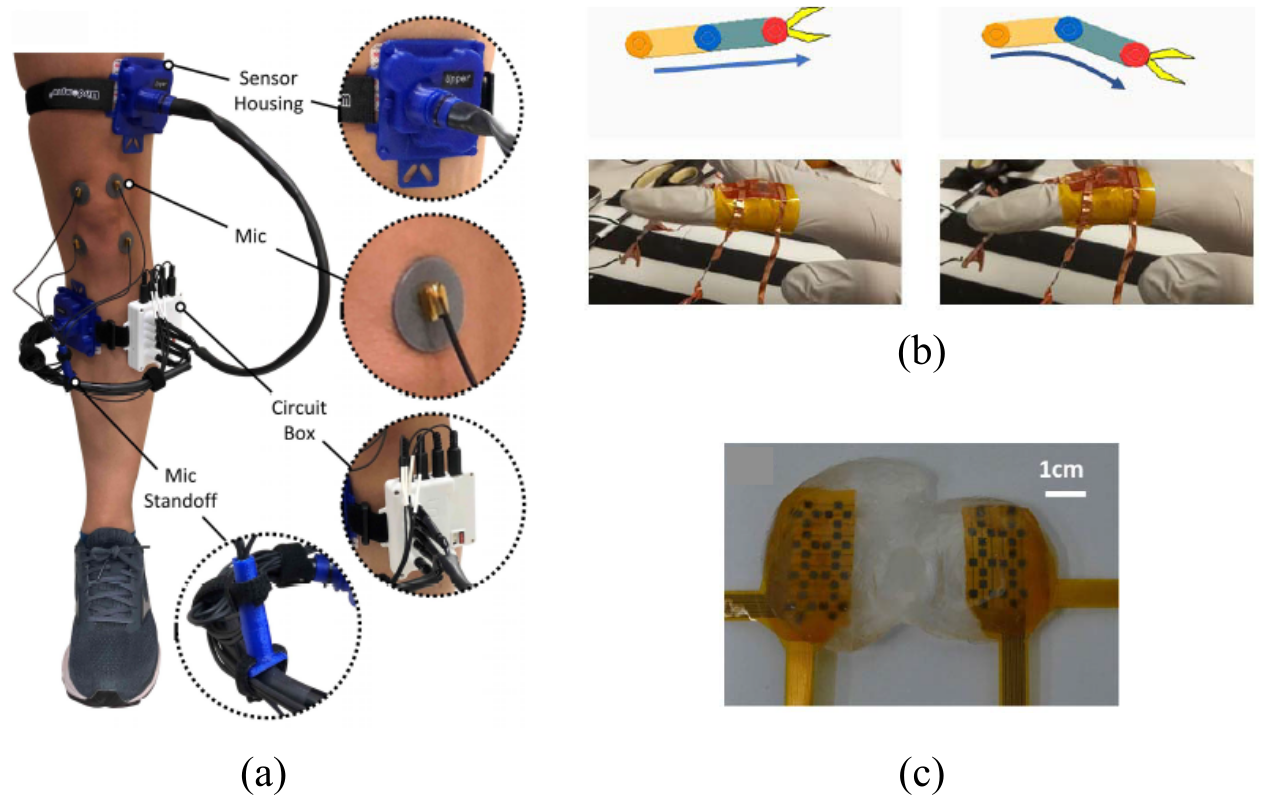
\includegraphics[scale=1]{Figure/Prosthetics/Prosthetics.png}
    \caption{Various assistive technologies used in prosthetics. (a) Wearable, multimodal sensor brace for knee joint health assessment, reproduced with permission from \parencite{teague_wearable_2020}.
     (b) A polymer microelectromechanical system-integrated flexible sensor, reproduced with permission from \parencite{fan_polymer_2019}.(c) A flexible pressure sensing device with bendable and distortable sensor arrays for force detection in knee arthroplasty, reproduced with permission from \parencite{sun_development_2020}.}
    \label{fig:Prosthetics}
\end{figure}

Another issue is the control of bionic hands. \textcite{alshammary_synergistic_2018} proposes using an inertial measurement unit (IMU) and electromyography (EMG) sensor for controlling a transhumeral myoelectric prosthesis, a type of bionic hand combined with a prosthetic forearm. The prosthetic system switches between hand- and elbow-based movement control dynamically according to the data from the IMU and the EMG sensors. The IMU on the forearm measures the angular velocity parallel to the elbow’s axis of rotation, and EMG electrodes on the upper to monitor muscular activity. When the elbow velocity is zero, and there is no upper arm activity, the control is given to the hand; when those parameters become non-zero again, the elbow takes control of the system. 



\subsection{Sensor in Use}
\subsubsection{Pressure Sensors}

Piezoresistive materials \parencite{sun_development_2020}, magnetic sensors \parencite{wu_skin-inspired_2018}, and MEMS-based sensors \parencite{fan_polymer_2019} are among the devices used for pressure sensing. The meniscus-shaped flexible pressure sensor in \textcite{sun_development_2020} is composed of polyimide (PI) electronic layers and nanocomposite sensing elements made of carbon nanotubes (CNT) and polydimethylsiloxane (PDMS). The size of the sensor is 2x2 $mm^2$ and it has a thickness of 400 $\mu$m. Due to the applied pressure, when deformation occurs on the sensing elements, the conductive channels  in CNTs increase. This reflects the external pressure change as a voltage variation at the sensor's output with 1\%/N sensitivity in the range of 10-100N.  

(Wu et al., 2018) makes use of PDMS as well for pressure detection. The sensor in \textcite{wu_skin-inspired_2018} is a PDMS chamber with magnetic particles deposited on top and an inductive sensing element located at the bottom of the chamber. An LC oscillation circuit is utilized as the sensing element. A 100-$\mu$m inductor wound around a coplanar waveguide of 60-$\mu$m thickness forms the inductor. With a force applied on the magnetic top layer (the sensing area is approximately $4x10^-5$ $m^2$), the distance between the the magnetic particles and the inductor changes, which in turn varies the LC oscillation frequency. The variations in the frequency can be translated into pressure changes of down to 10 $\mu$N. 

The MEMS device in \textcite{fan_polymer_2019} is another PDMS-based sensor that produces a variable current output proportional to the external pressure. The sensor is a $\mu$m-size capsule which top layer is encapsulated by a PDMS microstructure with three electrodes. When a pressure is applied on the capsule (whether on the top or bottom layers), the electrodes create contact with the patterned gold electrodes on the polyimide bottom layer. As the pressure increases, the quality of connection improves; therefore, the current flowing through the microstructure increases.

%%%%%%%%%%%%%%%%%%%%%%%%%%%%%%%%%%%%%%%%%%%%%%%%%%%%%%%%%%%%%%%%%%%%%%%%%%%%%%%%%%%%%%%%%%%%%%%%%%%%%%%%%%%%%%%%%%%%%%
